\subsection{Resultados}
\label{sec:results_AT_line}
%\subsubsection{Modelo AT con defecto en forma de línea}

Nuestro objetivo principal en el estudio del sistema AT con defecto es el de determinar la dependencia
 del exponente crítico de la función de correlación spin-spin $x_{corr}$ con la intensidad del acoplamiento entre los spines
 $\sigma$ y $\tau$ $K_{4}$. Como hemos mencionado en la sec. \ref{sec:teoria_escala} este exponente está directamente relacionado
 con el exponente crítico de la magnetización local de la línea de defectos $x_{m}$. Aprovechando esta conexión junto al hecho de que
 la determinación de este último exponente es más sencilla que la de $x_{corr}$, hemos realizado medidas de la magnetización sobre el defecto
 y a partir de ellas determinado el comportamiento de $x_{m}$.\\

Presentamos a continuación los resultados numéricos obtenidos en el estudio de la dependencia de
 $x_{m}^{\alpha}$ con la intensidad del defecto sobre la l\'inea E-F del diagrama de fases (Fig. \ref{fig:AT_ph_diag_Baxter}) definida por la ec. \ref{eq:lincrit}.
Los puntos sobre la l\'inea E-F pueden clasificarse seg\'un el valor del par\'ametro $\epsilon=K_{4}/K$, que representa el acoplamiento
 entre los spines $\sigma$ y los $\tau$:
$\epsilon<0$, los spines $\tau$ tienden a alinearse antiferromagnéticamente con los $\sigma$; $\epsilon=0$, no hay acoplamiento
 entre los $\tau$ y los $\sigma$; $\epsilon>0$, el acoplamiento es del tipo ferromagnético.
Al extremo E de la l\'inea E-F le corresponde el valor $\epsilon = -1$ en el l\'imite $K\rightarrow \infty$ y al punto F el valor $\epsilon = 1$.
 Una vez elegido el valor del par\'ametro $\epsilon$
 para una medida, los valores de $K_{4}$ y $K$ se determinan a  partir de la ec. \ref{eq:lincrit} y la relaci\'on $\epsilon=K_{4}/K$.\\

Debido al tamaño finito del sistema, el valor del exponente cr\'itico depende de $L$, y debe determinarse a partir de medidas de la magnetización para distintos tamaños,
 seg\'un la relación:

\begin{equation}
	\label{eq:magvsL}
	m_{l}^{\alpha}(L)\sim L^{-x_{m}^{\alpha}}, \; \; \; \; \alpha=\sigma , \tau .
\end{equation}
Hemos realizado medidas considerando tamaños hasta $L=128$ en una red cuadrada con condiciones de contorno periódicas.\\

\begin{figure}[h!]
\begin{center}
\includegraphics[width=\figwidth]{graf/exp/mls_vs_L_e0.eps}
\end{center}
\caption{Logaritmo de la magnetización sobre el defecto $m_{l}^{\sigma}$ en función del logaritmo del tamaño del sistema para diferentes valores de $K_{l}$,
la pendiente de estas rectas representa el valor del exponente cr\'itico $x_{m}^{\sigma}$.}
\label{fig:mls_vs_L_e0}
\end{figure}

\subsubsection{Sistema desacoplado: $\epsilon=0$}

Como ya hemos mencionado, en este caso el sistema se divide en dos modelos de Ising idenpendientes. Uno con un defecto en forma de l\'inea
 (spines $\sigma$) y otro que carece de defectos (spines $\tau$) y, por lo tanto, debe comportarse como el modelo de Ising bidimensional.
El resultado analítico para los exponentes $x_{m}^{\sigma}$ y $x_{m}^{\tau}$ (ec. \ref{eq:exp_crit_e0}) est\'a dado por:

\begin{equation*}
	\label{eq:exp_crit_e0}
	x_{m}^{\sigma} = \frac{2}{\pi^{2}}\arctan^{2}(e^{-2K_{l}}) , \; \; \; \; x_{m}^{\tau}=1/8, \; \; \; \; K_{4}=0
\end{equation*}

Dado que $\epsilon=0$, los resultados de esta secci\'on corresponden a los valores cr\'iticos de $K_{4}=0$ y $K=K_{c}^{Ising}$.
 mientras que para la intensidad del defecto hemos considerado diferentes valores entre $K_{l}=-0.4$ y $K_{l}=0.44$.
 Las medidas de la magnetizaci\'on sobre el defecto
 de los spines $\sigma$ en función de $L$ para estos valores de $K_{l}$ se muestran en la figura \ref{fig:mls_vs_L_e0} en escala logar\'itmica,
 claramente el comportamiento de $m_{l}$ se ajusta a una ley de potencias y los valores del exponente cr\'itico corresponden a la pendiente
 de cada una de las rectas (en este caso la dependencia del exponente con L es despreciable) . Los valores num\'ericos de dicho exponente en funci\'on de la intensidad del defecto se presentan en la Fig.
 \ref{fig:fit_arctan_e0}, donce puede verse que est\'an en completo acuerdo con el resultado anal\'itico (ec. \ref{eq:exp_crit_e0}),
 gr\'afico en l\'inea punteada.\\
En el caso de los spines $\tau$, el exponente cr\'itico $x_{m}^{\tau}$ es el mismo para todos los valores de $K_{l}$, y su valor coincide con el resultado
 conocido para el modelo de Ising sin defecto $x_{m}^{\tau}=\frac{1}{8}$.\\  

\begin{figure}[h!]
\begin{center}
\includegraphics[width=\figwidth]{graf/exp/fit_arctan_e0.eps}
\end{center}
\caption{Exponente crítico de la magnetización del defecto para $\epsilon=0$, la línea punteada representa el resultado teórico (\ref{eq:exp_crit_e0}).}
\label{fig:fit_arctan_e0}
\end{figure}

\subsubsection{Acoplamiento positivo: $\epsilon>0$}

Cuando el acoplamiento entre los spines $\sigma$ y los $\tau$, $\epsilon$, es diferente de cero, la magnetización del defecto
 no se comporta exactamente como una ley de potencias, es decir que los exponentes $x_{m}^{\sigma}$ y $x_{m}^{\tau}$ dependen del
 tamaño del sistema $L$. Hemos realizado medidas de la magnetizaci\'on sobre el defecto $m_{l}$ a fines de determinar la dependencia del
 exponente cr\'itico con el par\'ametro $\epsilon$. Todas estas medidas corresponden a puntos sobre la curva cr\'itica E-F
 en el plano ($K$, $K_{4}$), de forma que para una dado valor de $\epsilon$, $K$ y $K_{4}$ deben satisfacer la ec. \ref{eq:lincrit}.
 En la Fig. \ref{fig:desv} se observa la magnetización del defecto en función de $L$ (en escala logar\'itmica) para los casos
 $\epsilon=0$ y $\epsilon=0.75$, en el segundo caso puede apreciarse claramente una desviación respecto al comportamiento de una ley de potencias.

\begin{figure}[h!]
\begin{center}
\includegraphics[width=\figwidth]{graf/exp/desv_e0.75_vs_e0.eps}
\end{center}
\caption{Gráfico del logaritmo de $m_{l}^{\sigma}$ vs. el logaritmo de $L$ para una intesidad del defecto $K_{l}=-0.35$ en
 los casos $\epsilon=0$ y $\epsilon=0.75$, puede apreciarse la desviación respecto de una ley de potencias cuando $\epsilon\neq 0$.}
\label{fig:desv}
\end{figure}
Se espera que para valores muy grandes de $L$ la magnetización recupere su comportamiento como ley de potencias en función
 de $L$, y por lo tanto el exponente crítico efectivo tienda al valor correspondiente a un sistema de tamaño infinito,
 $x_{m}(L)\rightarrow x_{m}(\infty)$. Sin embargo el tamaño de sistema m\'aximo que puede ser alcanzado, manteniendo un tiempo de c\'alculo
 aceptable est\'a limitado, principalmente por la eficiencia del algoritmo utilizado cerca de las regiones cr\'iticas.
 
%Una primera aproximaci\'on al valor efectivo del exponente puede obtenerse a partir de la magnetización para dos valores diferentes
% del tamaño del sistema, $L$ y $bL$, tomando el logaritmo de la ec. (\ref{eq:magvsL}) y resolviendo para $x_{m}$:
%\\
%\begin{equation}
%	\label{eq:exp_eff}
%	x_{m}^{\alpha}(L) = \frac{\ln{m_{l}^{\alpha}(bL)}-\ln{m_{l}^{\alpha}(bL)}}{\ln{b}}, \; \; \; \; \alpha=\sigma , \tau .
%\end{equation}
%\\
Hemos considerado tres valores positivos diferentes de $\epsilon$, para cada uno de ellos medimos la magnetizaci\'on sobre el
 defecto para diferentes intensidades del defecto $K_{l}$. La figura \ref{fig:ml_vs_L_all}
 muestra gr\'aficos del logaritmo de $m_{l}^{\alpha}$ en funci\'on del logaritmo de $L$, por lo tanto la pendiente de estas curvas
 representa el exponente crítico efectivo $x_{m}^{\alpha}(L)$, ya que tomando el logaritmo de la ec.(\ref{eq:magvsL}), que lo define, se obtiene:
 
\begin{equation}
	\label{eq:logmagvsL}
	\ln{(m_{l}^{\alpha}(L))} \sim -x_{m}^{\alpha}\Ln{(L)}, \; \; \; \; \alpha=\sigma , \tau .
\end{equation}
 
\begin{figure}[h!]
\begin{center}
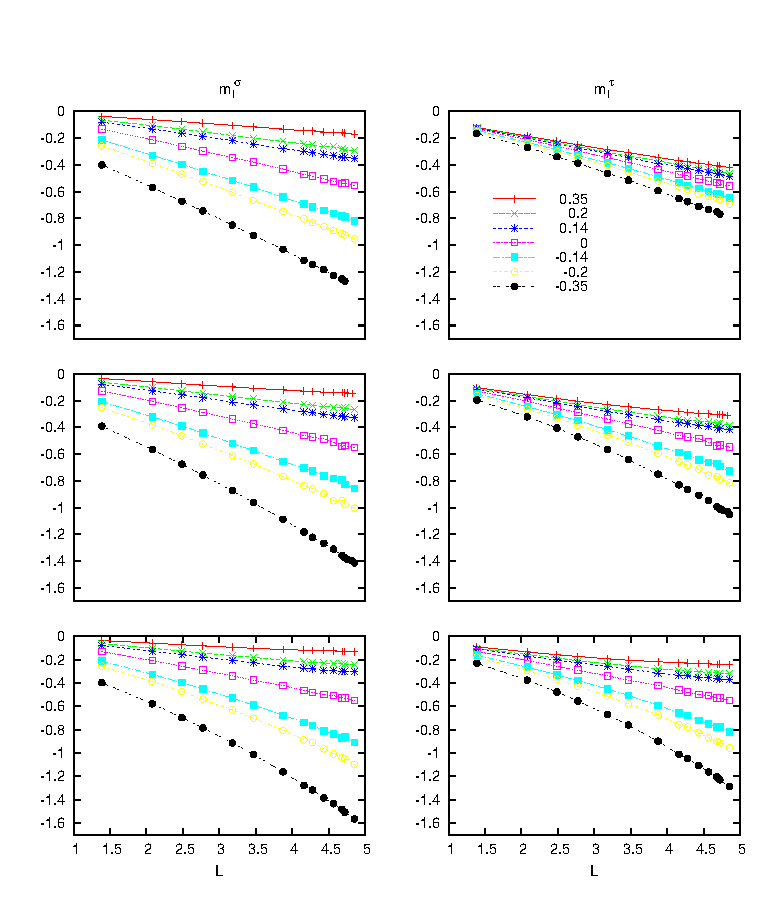
\includegraphics[width=\figwidth]{graf/exp/ml_vs_L_all.eps}
\end{center}
\caption{Gráfico del logaritmo de la magnetización sobre el defecto $m_{l}^{\alpha}$ en función del logaritmo del tamaño del
 sistema $L$. Cada fila corresponde a un valor diferente del acoplamiento entre los spines $\sigma$ y los $\tau$,
 $\epsilon=0.25, 0.5, 0.75$. En la columna de la izquierda se representan los datos para los spines $\sigma$ y en
 la columna derecha para los $\tau$. Cada uno de estos gr\'aficos contiene las medidas de $m_{l}^{\alpha}$ para cinco
 valores diferentes de la intensidad del defecto $K_{l}=-0.35, -0.2, -0.14, 0, 0.14, 0.2, 0.35$. La pendiente de las
 curvas disminuye para valores positivos de $K_{l}$ (s\'imbolos \textcolor{red}{$+$}, \textcolor{green}{$\times$}
 y \textcolor{blue}{$\times$}) y aumenta para los valores negativos de $K_{l}$ (\textcolor{cyan}{$\square$}, \textcolor{yellow}{$\circ$}
 y $\bullet$).}
\label{fig:ml_vs_L_all}
\end{figure}
Los resultados se presentan en un arreglo en el que la columna de la izquierda corresponde a los spines $\sigma$,
 la de la derecha a los $\tau$ y cada fila a un valor diferente de $\epsilon$ en orden creciente hacia abajo,
 $\epsilon=0.25,0.5,0.75$. Cada uno de los gr\'aficos contiene las curvas para cinco valores diferentes de $K_{l}$.
 Las tres curvas de menor pendiente en cada gr\'afico son para los valores  positivos de la intensidad del defecto
 (s\'imbolos \textcolor{red}{$+$}, \textcolor{green}{$\times$} y \textcolor{blue}{$*$}), en estos casos la
 pendiente disminuye a medida que aumenta el tamaño del sistema, por lo tanto el exponente
 $x_{m}^{\alpha}$ tiende a un valor $x_{m>}^{\alpha}$ menor al correspondiente al sistema libre de defectos, tanto para los espines
 $\tau$ como para los $\sigma$, y la desviación respecto del valor sin defectos aumenta a medida que el valor de $K_{l}$ se aparta de $0$.
 %Se espera que, para valores muy grandes de $L$, $x_{m>}^{\alpha}$ se aproxime a cero.
La curva central (\textcolor{magenta}{$\square$}) corresponde a $K_{l}=0$, tiene en todos los casos una pendiente muy pr\'oxima
 a $\frac{1}{8}$ y pr\'acticamente no muestra desviaciones de este valor al aumentar $L$.
Las tres curvas inferiores de cada gr\'afico, las de mayor pendiente, corresponden a valores negativos de la intensidad del defecto,
 en este caso el exponente crítico se aproxima a un valor $x_{m<}^{\alpha}$ mayor a $\frac{1}{8}$ y la desviación respecto al caso desacoplado
 es también más apreciable para los valores más negativos de $K_{l}$.\\

Los valores num\'ericos del exponente cr\'itico efectivo pueden obtenerse a partir de la magnetización para dos
 valores diferentes del tamaño del sistema, $L$ y $bL$, tomando el logaritmo de la ec. (\ref{eq:magvsL}) y resolviendo para $x_{m}$:
\begin{equation}
	\label{eq:exp_eff}
	x_{m}^{\alpha}(L) = \frac{\ln{m_{l}^{\alpha}(bL)}-\ln{m_{l}^{\alpha}(bL)}}{\ln{b}}, \; \; \; \; \alpha=\sigma , \tau .
\end{equation}

Si se grafican los valores obtenidos en funci\'on de la inversa del tamaño del sistema, $\frac{1}{L}$, el valor
del exponente en el l\'imite $L\rightarrow \infty$ puede estimarse determinando graficamente la intersecci\'on
de la extrapolaci\'on de la gr\'afica con la l\'inea vertical $L=0$. En nuestro caso, debido a la lenta convergencia
del algoritmo utilizado en la regi\'on cr\'itica, la extrapolaci\'on mencionada es muy dif\'icil de realizar. Por ejemplo, la Fig.\ref{fig:xfits}
muestra la gr\'afica obtenida de esta forma para $\epsilon=0.75$ y $K_{l}=-0.35$ donde se aprecian las fluctuaciones para L grande.
 Por ello hemos optado por determinar el
valor del exponente cr\'itico para el mayor valor del tamaño del sistema $L=128$ utilizado en las simulaciones ajustando un polinomio de orden $2$
a la gr\'afica de $\ln{(m_{l})}$ vs. $L$ (Fig. \ref{fig:xfits}-(a)), a partir del cual obtenemos el valor del exponente
evaluando la derivada en $L=128$. Mediante este procedimiento determinamos $x_{m}$ para todos los valores de $\epsilon$
y $K_{l}$ estudiados.
Su comportamiento se muestra en la Fig. \ref{fig:exps_st_all}
 para los tres valores de $\epsilon$ como funci\'on de $K_{l}$. Se incluyen
 tambi\'en con fines comparativos los datos para $\epsilon=0$ y el resultado te\'orico para ese mismo caso. La desviaci\'on
 respecto al caso desacoplado aumenta con la intensidad del acoplamiento $\epsilon$ y es mas fuerte para el exponente asociado
 a los spines $\sigma$ (s\'imbolos sin relleno en la figura, $\vartriangle$, $\circ$ y $\square$) que para el exponente $x_{m}^{\tau}$ asociado a los $\tau$
 (s\'imbolos $\blacktriangle$, $\bullet$ y $\blacksquare$).
Para valores positivos de $K_{l}$, $x_{m}^{\sigma,\tau}$ tiene un valor menor al que presenta para $K_{l}=0$, y se aproxima
 a cero a medida que $K_{l}$ aumenta.
Para valores negativos de $K_{l}$, los exponentes cr\'iticos son mayores que para el caso sin defecto y aumentan a medida que el
 valor absoluto de $K_{l}$ crece.\\
 
\begin{figure}[htbp!]
\begin{center}
\includegraphics[width=\figwidth]{graf/exp/mag_exp_e0.75_Jln0.35.eps}
\end{center}
\caption{(a) Magnetizaci\'on sobre el defecto en funci\'on de la inversa del tamaño del sistema, $\frac{1}{L}$ para
 $\epsilon=0.75$ y $K_{l}=-0.35$, la l\'inea punteada muestra el ajuste de un polinomio de grado $2$, (b) valor efectivo
  del exponente cr\'itico de la magnetizaci\'on obtenido utilizando la ec.(\ref{eq:exp_eff})
 para los puntos de la gr\'afica (a) tomados de a pares.}
\label{fig:xfits}
\end{figure}

\begin{figure}[h!]
\begin{center}
\includegraphics[width=\figwidth]{graf/exp/exp_all_01.eps}
\end{center}
\caption{Exponente crítico de la magnetización del defecto, en función de la intensidad $K_{l}$. Se muestran los resultados para $\epsilon=0.25,0.5,0.75$.
Los puntos del gráfico representados por símbolos sin relleno $\vartriangle$, $\circ$ y $\square$ corresponden a los spines $\sigma$, mientras que los 
representados por símbolos rellenos, $\blacktriangle$, $\bullet$ y $\blacksquare$, corresponden a los spines $\tau$. La línea horizontal punteada
indica el valor $\frac{1}{8}$, valor teórico del exponente para $K_{l}=0$.}
\label{fig:exps_st_all}
\end{figure}

El hecho de que el valor del exponente se aproxime a cero cuando la intensidad del defecto es grande y positiva, puede ser analizado
 en terminos de la transici\'on de fase orden-desorden para la l\'inea de defectos. Los spines que yacen sobre la l\'inea
 se encuentran acoplados entre s\'i por una constante efectiva $K_{ef}=K+K_{l}$ que es m\'as fuerte que su acoplamiento
 con los \'atomos que no est\'an sobre la l\'inea, es decir sus vecinos en la direcci\'on perpendicular a ésta. De esta forma,
 el defecto tiende a estar ordenado para valores de $K$ menores al valor cr\'itico para el plano, y se encuentra en ese estado cuando
 el resto del sistema transita del desorden al orden. Este comportamiento puede verse en la figura \ref{fig:line_enhdec3_e0.75}, donde
 se muestran los par\'ametros de orden $\mean{\sigma}$ y $\mean{\sigma}_{l}$ que miden el orden del plano formado por todos los spines
 de tipo $\sigma$ y de la l\'inea de defectos, respectivamente, en funci\'on del acoplamiento $K$, para una transici\'on de fase sobre
 la curva E-F.\\

\begin{figure}[h!]
\begin{center}
\includegraphics[width=\figwidth]{graf/exp/line_enhdec3_e0.75.eps}
\end{center}
\caption{Parámetros de orden $\mean{\sigma}$ (magnetizaci\'on del plano $\sigma$) y $\mean{\sigma}_{l}$ (magnetizaci\'on sobre el defecto)
 para una transici\'on de fase sobre la l\'inea E-F. Cuando la intensidad del defecto es positiva $K_{l}=0.35$, la l\'inea se ordena
 para valores de $K$ inferiores al valor cr\'tico para el plano. Es decir que se encuentra ordenada cuando ocurre la transici\'on para el plano.
 Cuando $K_{l}=-0.35$ la l\'inea est\'a desordenada durante la transici\'on de fase.}
\label{fig:line_enhdec3_e0.75}
\end{figure}

Siguiendo el mismo razonamiento para el caso en que la intensidad del defecto es negativa, el valor efectivo del acoplamiento entre \'atomos sobre
 el defecto es menor que el acoplamiento $K$ y en consecuencia la l\'inea de defectos se encuentra desordenada o en transici\'on al orden para el
 valor de $K$ que produce el ordenamiento del plano.\\

\subsubsection{Acoplamiento negativo: $\epsilon<0$}

Observando las gr\'aficas del logaritmo de la magnetizaci\'on en funci\'on del logaritmo de $L$ cuando $\epsilon$ es negativo (figura \ref{fig:ml_vs_L_neg_all})
 podemos ver que en este caso el comportamiento para los spines $\sigma$ es diferente que para los $\tau$.\\
Para los $\sigma$ ocurre
 lo mismo que en el caso $\epsilon>0$, la pendiente del logaritmo de la magnetizaci\'on para valores positivos del defecto
 es menor que para el caso libre de defecto, mientras que para un defecto con intesidad negativa la pendiente es mayor. Para los
 spines $\tau$, sin embargo el comportamiento es inverso, es decir, las pendientes son mayores cuando la intesidad del defecto
 es positiva y menores cuando es negativa.
La figura \ref{fig:exp_neg_e0.75}, muestra los exponentes cr\'iticos $x_{m}^{\sigma}$ y $x_{m}^{\tau}$, obtenidos mediante ajustes
 de segundo orden al igual que en el caso $\epsilon>0$, como funci\'on de la intensidad del defecto.\\


\begin{figure}[h!]
\begin{center}
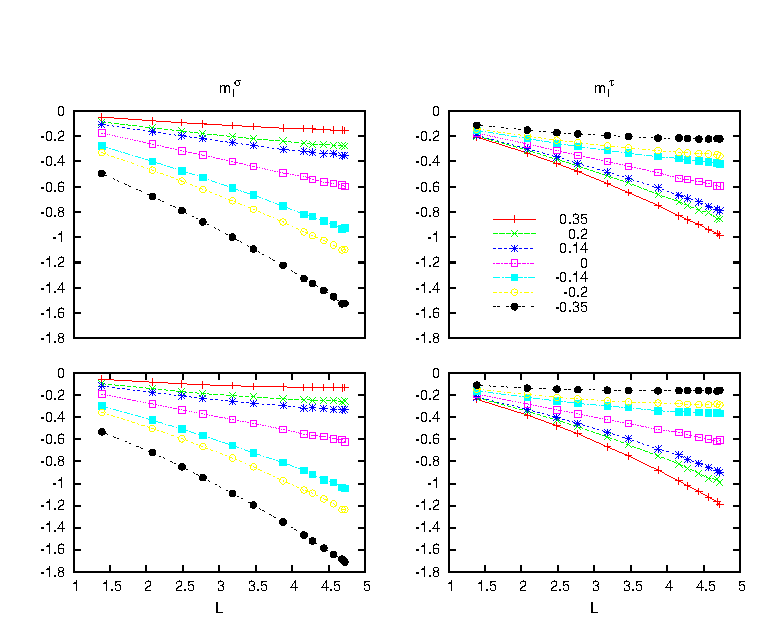
\includegraphics[width=\figwidth]{graf/exp/ml_vs_L_neg_all.eps}
\end{center}
\caption{Gráfico en escala logarítmica de la magnetización sobre el defecto $m_{l}^{\alpha}$ en función el tamaño del sistema $L$. Cada fila corresponde
 a un valor diferente del acoplamiento ($\epsilon=-0.5, -0.75$) entre los spines $\sigma$ y los $\tau$. En la columna de la izquierda se representan
 los datos para los spines $\sigma$ y en la columna derecha para los $\tau$.}
\label{fig:ml_vs_L_neg_all}
\end{figure}

\begin{figure}[h!]
\begin{center}
\includegraphics[width=\figwidth]{graf/exp/exp_all_neg_01.eps}
\end{center}
\caption{Exponente crítico de la magnetización del defecto, en función de la intensidad $K_{l}$ para $\epsilon <0$. Se muestran los resultados
 para $\epsilon=-0.5,-0.75$. Los puntos representados con símbolos sin relleno corresponden a los spines $\sigma$, su comportamiento es similar
 al hallado para valores positivos de $\epsilon$. El comportamiento del exponente asociado a los spines $\tau$ es contrario al hallado para
 $\epsilon>0$, estos valores están representados con símbolos rellenos.}
\label{fig:exp_neg_e0.75}
\end{figure}
